
\begin{frame}{第一讲、集合与映射}
	\linespread{1.5}
	\begin{enumerate}
	  \item {\bf 内容与要求}{\color{blue}( \S1.1)}
	  \begin{itemize}
	    \item 理解集合的概念、运算及其性质
	    \item 了解实数集的一些重要性质
	    \item 理解映射的概念
	  \vspace{1em}
	  \end{itemize}
	  \item {\bf 课后练习:}
	  \begin{itemize}
	    \item 书面作业:{\b 习题1.1:4(2),9,12}
	    \item 思考题:{\b 习题1.1:7,8,10,13,14}
	  \end{itemize}
	\end{enumerate}
\end{frame}

\section{集合}

\begin{frame}{什么是集合?}
	\linespread{1.2}\pause 
	\begin{block}{Cantor(1845-1918)}
		所谓{\b 集合},是指把一些个体({\b 元素})\pause 放在一起考虑时它们形成的整体。
	\end{block}\pause 
	\begin{itemize}
	  \item 满足一定性质的所有个体\pause :$A=\{x|x$满足性质$P\}$\pause 
	  \item 列举法\pause :$A=\{$足球,橘子,老师,计算机$\}$
	\end{itemize}\pause 
	\begin{block}{Poincare,1900,国际数学家大会}\pause 
		 \alert{“\ldots 借助集合论概念,我们可以建造整个数学大厦\ldots \pause 今天,我们可以说绝对的严格性已经达到了\ldots”}
	\end{block}
\end{frame}

\begin{frame}{常见的集合}
	\linespread{1.4}\pause 
	\begin{enumerate}
	  \item {\b$\mathbb{N}$}:自然数集\pause 
	  \item {\b$\mathbb{Z}$}:整数集(所有自然数及其相反数,$0$)\pause 
	  \item {\b$\mathbb{Q}$}:有理数集($p/q,\,(p,q\in\mathbb{Z},q\ne 0)$)\pause 
	  \item {\b$\mathbb{R}$}:\alert{实数集}(无理数:有理数集的分割)\pause 
	  \item {\b$\mathbb{C}$}:复数集(有序实数对)\pause 
	\end{enumerate}
	\linespread{1.2}
	{\bf 注:}通过集合的笛卡尔乘积{\b “$\times$”}\pause 可以定义更\alert{“高维”}的集合,\pause 例如:\\
	\centerline{$\mathbb{R}^2=\mathbb{R}\times\mathbb{R}$}
\end{frame}

\begin{frame}{罗素悖论(Russell Paradox)*}
	\linespread{1.2}\pause 
	\begin{block}{Russell, 1901}
		只给不给自己理发的人理发的理发师该不该给自己理发?
	\end{block}\pause 
	设$x\in A$表示:$A$给$x$理发,\pause 定义
	$$A=\{x|x\notin x\},$$\pause 
	问:$A\in A$还是$A\notin A$?\pause 
% 	\ba{罗素悖论导致了第三次“数学危机”的出现!}
	\begin{block}{{\ba{第三次“数学危机”}}(Frege,1901,《算术基础》)}
		“在工作结束之后发现那大厦的基础已经动摇,对于一个科学工作者来说,没有比这更不幸的了”
	\end{block}
\end{frame}

% \begin{frame}{罗素悖论(Russell Paradox)}
% 	\linespread{1.2}\pause 
% 	\begin{block}{Russell, 1901}
% 		只给别人理发的理发师应不应该给自己理发?
% 	\end{block}\pause 
% 	将所有集合分为两类\pause 
% 	$$P=\{A|A\in A\},\pause \quad Q=\{A|A\notin A\},$$\pause 
% 	问:$Q\in Q$还是$Q\notin Q$成立?\pause 
% % 	\ba{罗素悖论导致了第三次“数学危机”的出现!}
% 	\begin{block}{{\ba{第三次“数学危机”}}(Frege,1901,《算术基础》)}
% 		“在工作结束之后发现那大厦的基础已经动摇,对于一个科学工作者来说,没有比这更不幸的了”
% 	\end{block}
% \end{frame}

\begin{frame}{问题出在哪里?}
	\linespread{1.2}\pause 
	\begin{block}{{\bf 无限抽象原则}(Cantor,Frege)}\pause 
		任意给定某个条件就可以确定一个集合。\pause (每个概念的外延可以确定一个集合)
	\end{block}\pause 
	{\bf 观点:}不加限制地使用无限抽象原则将导致罗素悖论\pause 
	\begin{block}{{\bf 有限抽象原则}(限制公理)}\pause 
		如果已知一个集合\pause 和一个给定的条件,\pause 则该集合中所有满足条件的元素{\b 可以}构成一个集合。
	\end{block}\pause 
	\ba{ZFS(Zermelo-Fraenkel-Skolem)公理化集合系统}
\end{frame}

\begin{frame}{公理系统*}
	\linespread{1.2}\pause 
	\begin{block}{公理(Axiom)}\pause 
		无须证明即为正确的命题。
	\end{block}\pause 
	\begin{itemize}
	  \item {\bf Engles:}数学上的所谓公理,是数学需要用作自己出发点的少数思想上的规定\pause 
	  \item {\bf ZFS系统:}公理就是一些关于逻辑符号\alert{“$\in$”}和\alert{字母}的组合使用方法的约定\pause 
	  \item {\b 公理化方法}是构建现代数学理论体系的基石\pause 
	\end{itemize}
	\vspace{1ex}
	\centerline{\Large\ba{数学就等于永恒的真理吗?}}
\end{frame}

\section{实数集}

\begin{frame}{实数集的一些重要性质}
	\linespread{1.5}
	\begin{enumerate}\pause 
	  \item {\bf 有序性:\pause }任意两个实数均可比较大小\pause 
	  \item {\bf 完备性:\pause }实数集与数轴上的点之间存在一一对应\pause 
	  \item {\ba{连续性公理(确界原理):}}非空有{\b 上界}的实数集必有{\b 上确界}\pause 
	  \begin{itemize}
	    \item {\bf 上确界:}最小的上界!\pause 
	  \end{itemize}
	\end{enumerate}
	{\bf 注:}有理数集不满足连续性公理\pause ,即:有理数集的上(下)确界未必是有理数。
\end{frame}

\begin{frame}{$e=\mathrm{sup}\left\{\left(1+\frac
1n\right)^n\right|n\in\mathbb{N}\}\notin\mathbb{Q}$}
	\linespread{1.2}\pause
	\begin{center}
		\resizebox{!}{6cm}{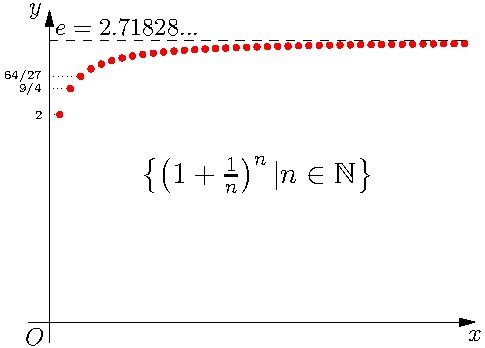
\includegraphics{./images/ch1/e-notin-N.pdf}}
% 		\resizebox{!}{4.8cm}{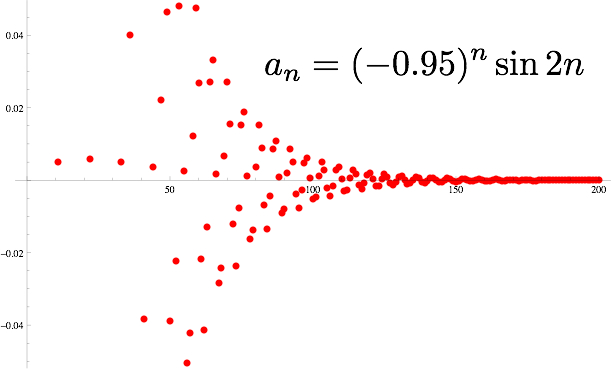
\includegraphics{./images/ch2/sin2nn.jpg}}
% 		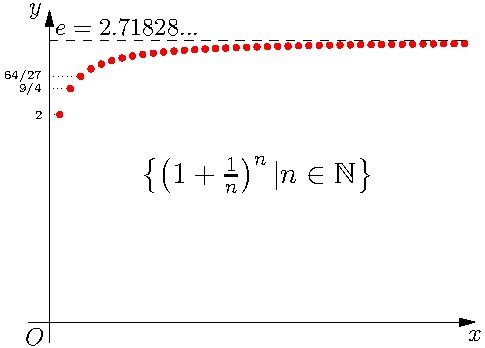
\includegraphics[width=6cm]{./images/ch1/e-notin-N}
	\end{center}\pause
	{\small
	$$\left(1+\frac11\right)^1<\left(1+\frac12\right)^2<\left(1+\frac13\right)^3<\ldots
	\left(1+\frac1n\right)^n<\ldots<e$$}
\end{frame}

\section{映射}

\begin{frame}{映射}
	\linespread{1.2}\pause 
	\begin{block}{教材P7}
		事物之间“一对一”或“多对一”的依赖关系
	\end{block}\pause 
	设集合$A,B$非空,\pause 若对任意$x\in
	A$,\pause 依照某种对应关系$f$,\pause 都存在$B$中的唯一元素$y$与之对应,\pause
	则称$f$是$A$到$B$的一个映射,\pause 记为: $f:A\to B$
	\begin{itemize}\pause 
	  \item {\bf 单射:\pause }$x_1\ne x_2\Rightarrow f(x_1)\ne f(x_2)$
	  \item {\bf 满射:\pause }$B$中任意元素都可在$A$中找到对应元素
	  \item {\bb 一一映射(双射):\pause }既是单射,又是满射
	\end{itemize}
\end{frame}

\begin{frame}{一一映射与无穷集合}
	\linespread{1.2}\pause 
	{\ba{问题:}}如何比较两个集合中元素的个数?\pause 
	\begin{exampleblock}{\bf 例}
		\begin{enumerate}\pause 
		  \item 自然数与正偶数一样多?\pause (\alert{$\surd$})\pause 
		  \item 自然数与整数一样多?\pause (\alert{$\surd$})\pause 
		  \item 自然数与有理数一样多?\pause (\alert{$\surd$})\pause 
		  \item 区间$(a,b)$中的实数与$\mathbb{R}$中一样多?\pause (\alert{$\surd$})\pause 
		  \item 自然数与实数一样多?\pause (\alert{$\times$})\pause 
		\end{enumerate}
	\end{exampleblock}\pause
	\begin{alertblock}{\bf 无穷集合}\pause 
		可以和自身的某个子集建立起一一映射的集合
	\end{alertblock}
\end{frame}

\begin{frame}[<+->]{小结}
	\linespread{1.5}
	\begin{enumerate}
	  \item {\bf 集合的概念与公理化方法}*
	  \item {\bf 映射}
	  \begin{itemize}
	    \item 一一映射与无穷集合
	  \end{itemize}
	\end{enumerate}
	\pause
% 	\vspace{1em}
	\pause
	\begin{exampleblock}{课后习题}
	  \begin{itemize}
	    \item 书面作业:{\b 习题1.1:4(2),9,12}
	    \item 思考题:{\b 习题1.1:7,8,10,13,14}
	  \end{itemize}
	\end{exampleblock}
\end{frame}

% \begin{frame}[<+->]{作业书写要求}
% 	\linespread{1.2}
% 	\begin{itemize}
% 	  \item 标明作业布置时间
% 	  \item 抄题,写清题目编号、页码
% 	  \item 不允许使用铅笔书写,画图除外
% 	  \item 字迹尽可能工整、清晰,数学符号书写规范
% 	  \item 段首缩进
% 	  \item 公式居中书写,独立成行
% 	  \item 作业纸不允许分栏使用
% 	  \item \ldots\ldots
% % 	  \item 两题之间空一行
% 	\end{itemize}
% \end{frame}

\begin{frame}{关于ZFS}
	\linespread{1.4}
	{\bf 命题:}在ZFS中,无法定义包含所有集合的集合。
	
	{\bf 证明:}反证法。设$A$是一个这样的集合。定义
	$$B=\{x\in A|x\notin x\}$$
	若
	$B\in A$,则必有$B\in B$或$B\notin B$。而若$B\in B$,可推出$B\notin B$;同理,
	由$B\notin B$,也可推出$B\in B$。从而$B\notin A$,推出矛盾。这说明$B$的定义存在问题,故知假设错误。
\end{frame}